\chapter{AspectJ Code Generation}
\label{chapter:codeGeneration}

\begin{flushright}
\textit{Chapter written by Claas Wilke}
\end{flushright}

This chapter describes how the Java Code Generator \keyword{OCL22Java} provided 
with Dresden OCL can be used. A general introduction into Dresden OCL can 
be found in Chapter~\ref{chapter:introduction}. A detailed documentation of the 
development of OCL22Java can be found in the Minor Thesis (Gro�er Beleg) of 
Claas Wilke~\cite{GB:Wilke}.

In addition to the general Eclipse installation the \keyword{\acf{AJDT}} are 
required to execute the code generated with OCL22Java. The \acs{AJDT} plug-ins
can be found at the \acs{AJDT} website~\cite{WWW:AJDT}.
  


\section{Code Generator Preparation}

This chapter uses the \keyword{Simple Example} which is provided with 
Dresden OCL and has been introduced in Section~\ref{intro:simpleExample}. Since
for this scenario we require two different projects and not just the one
imported in Chapter~\ref{chapter:introduction}, we use another example wizard
now. By using the menu option \emph{File -> New -> Dresden OCL Examples ->
Simple Example (Ocl22Java)} the two projects are imported into the Eclipse
workspace. Afterwards, the workspace should contain two projects named  
\model{org.dresdenocl.\linebreak[0]examp\-les.\linebreak[0]simple} and
\model{\ldots simple.\linebreak[0]ocl\-2\-2\-ja\-va\-code}
(cf. Fig.~\ref{pic:example:simple03}).

\begin{figure}[!t]
	\centering
	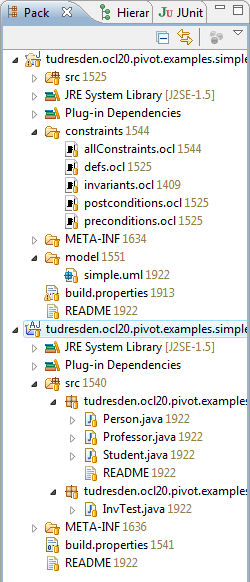
\includegraphics[width=0.4\linewidth]{figures/examples/simple03}
	\caption{The two projects which are required to run this tutorial.}
	\label{pic:example:simple03}
\end{figure}

The first project provides a model file which contains the simple class diagram
which has been explained in Section~\ref{intro:simpleExample} (the model file
is located at \model{model/simple.uml}) and the constraint file we want to
generate code for (the constraint file is located at
\model{constraints/invariants.ocl}). Listing~\ref{lst:codegen:simpleInvariant}
shows one invariant that is contained in the constraint file. The invariant 
declares that the \model{age} of any \model{Person} must be greater or equal 
to zero at any time during the life cycle of the \model{Person}.

\begin{figure}[!htbp]
	\centering
	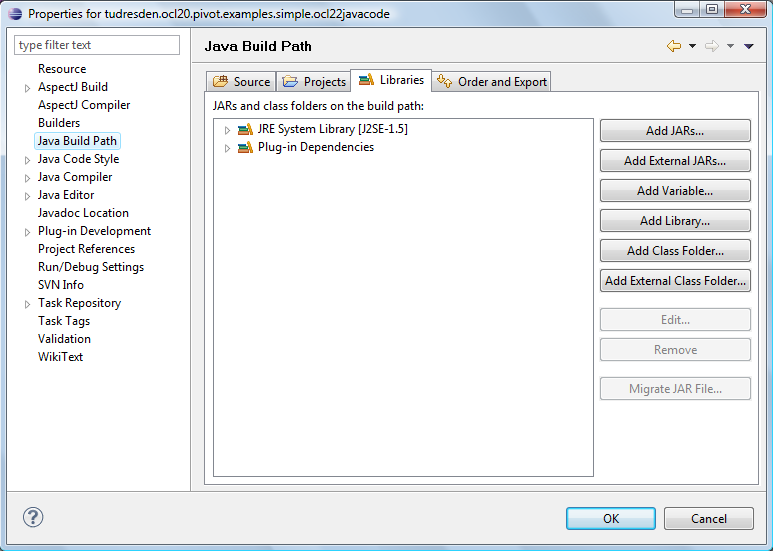
\includegraphics[width=1.0\linewidth]{figures/codegen/properties2}
	\caption{Adding a new library to the build path.}
	\label{pic:codegen:properties2}

  \vspace{2.0em}
  
  \lstset{
    language=OCL
  }
  \begin{lstlisting}[caption={A simple invariant.}, captionpos=b, label=lst:codegen:simpleInvariant]
-- The age of a person can not be negative.
context Person
inv: age >= 0
  \end{lstlisting}
  
  \vspace{2.0em}

  \centering
	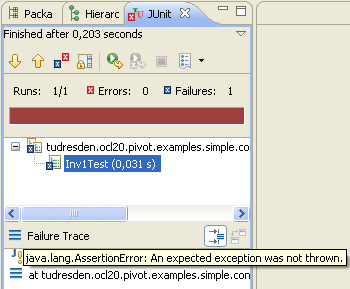
\includegraphics[width=0.6\linewidth]{figures/codegen/junit01}
	\caption{The result of the JUnit test case.}
	\label{pic:codegen:junit01}

\end{figure}

The second project provides the test class 
\model{src/org.dresdenocl.examples.simple.\linebreak[0]con\-straints.\linebreak[0]InvTest.java}
which contains a JUnit test case that checks, whether or not the mentioned
constraint is enforced during run-time. The test case creates two
\model{Persons} and tries to set their \model{age}. The \model{age} of the
second \model{Person} is set to \model{-3} and thus, the constraint is
violated. The test case expects that a run-time exception is thrown, if the
constraint is violated.

The code for the mentioned constraint has not been generated, yet and thus, the 
exception will not be thrown. We run the test case by opening the context menu 
on the Java class in the \eclipse{Package Explorer} and selecting the menu item
\eclipse{Run as -> JUnit Test}. The test case fails because the exception is not
thrown (cf. Fig.~\ref{pic:codegen:junit01}). To fulfill the test case we have 
to generate the ApsectJ code for the constraint which enforces the constraint's 
condition. How to generate such code will be explained in the following.


\newpage
\section{Code Generation}

To prepare the code generation we have to import the model 
\model{model/simple.uml} into the \eclipse{Model Browser}. We use the model
import wizard of Dresden OCL to import the model. This procedure is explained in
Chapter~\ref{chapter:introduction}. Afterwards, we have to open the constraint
file \model{con\-straints/\linebreak[0]in\-va\-riant.ocl}. Afterwrds, the
\eclipse{Model Browser} should look like illustrated in
Figure~\ref{pic:codegen:modelBrowser}. Now we can start the code generation.

\begin{figure}[!b]
	\centering
	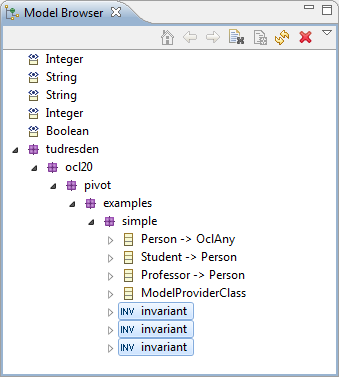
\includegraphics[width=0.6\linewidth]{figures/codegen/modelBrowser}
	\caption{The Model Browser containing the Simple Model and its constraints.}
	\label{pic:codegen:modelBrowser}
\end{figure}

To start the code generation we open the menu \eclipse{Dresden OCL} and select 
the item \eclipse{Generate AspectJ Constraint Code}.


\newpage
\subsection{Selecting a Model}

A wizard opens and we have to select a model for code generation (cf. 
Fig.~\ref{pic:codegen:codegen01}). We select the \model{simple.uml} model and
click the \eclipse{Next} button.

\begin{figure}[!b]
	\centering
	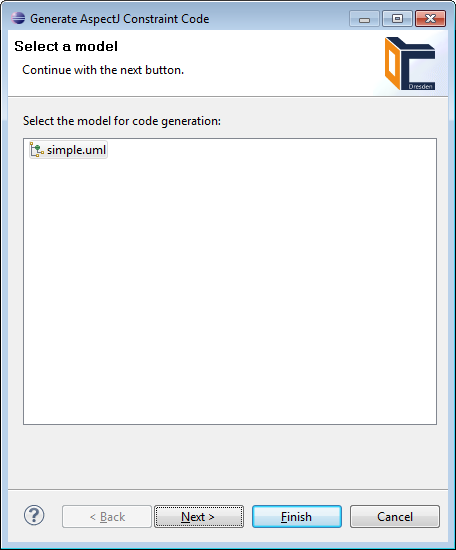
\includegraphics[width=0.9\linewidth]{figures/codegen/codegen01}
	\caption{The first step: selecting a model for code generation.}
	\label{pic:codegen:codegen01}
\end{figure}


\newpage
\subsection{Selecting Constraints}

As a second step we have to select the constraints for which we want to generate
code. We only select the constraint that enforces that the \model{age} of any 
\model{Person} must be equal to or greater than zero and click the 
\eclipse{Next} button (cf. Fig.~\ref{pic:codegen:codegen02}).

\begin{figure}[!b]
	\centering
	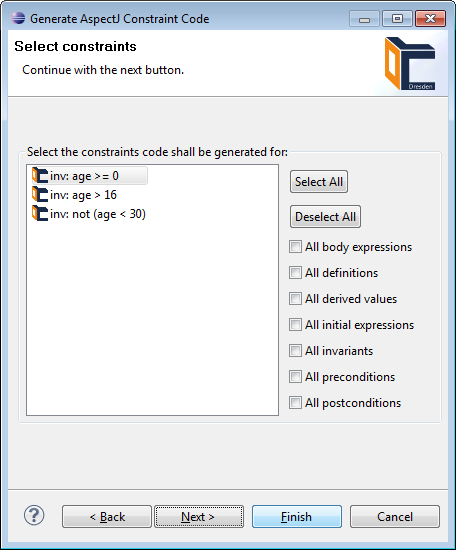
\includegraphics[width=0.9\linewidth]{figures/codegen/codegen02}
	\caption{The second step: selecting constraints for code generation.}
	\label{pic:codegen:codegen02}
\end{figure}


\newpage
\subsection{Selecting a Target Directory}

Next, we have to select a target directory into that the generated code shall 
be stored. We select the source directory of our second project (which is 
\model{tudresden.\linebreak[0]ocl20.pivot.examples.simple.\linebreak[0]ocl22javacode/src})
(cf. Fig.~\ref{pic:codegen:codegen03}). Please note, that we select the 
source directory and not the package directory into which the code shall be 
generated! The code generator creates or uses contained package directories 
depending on the package structure of the selected constraint. Additionally we
can specify a subfolder into that the constraint code shall be generated 
relatively to the package of the constrained class. By default this is a sub 
directory called \model{constraints}. We do not want to change this setting and
click the \eclipse{Next} button.
	
\begin{figure}[!b]
	\centering
	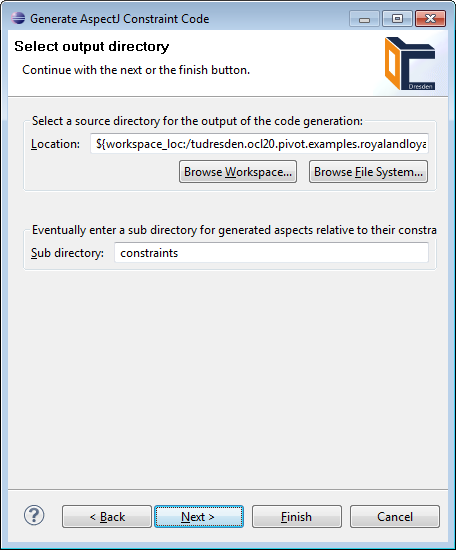
\includegraphics[width=0.9\linewidth]{figures/codegen/codegen03}
	\caption{The third step: selecting a target directory for the generated code.}
	\label{pic:codegen:codegen03}
\end{figure}


\newpage
\subsection{Specifying General Settings}
	
\begin{figure}[!b]
	\centering
	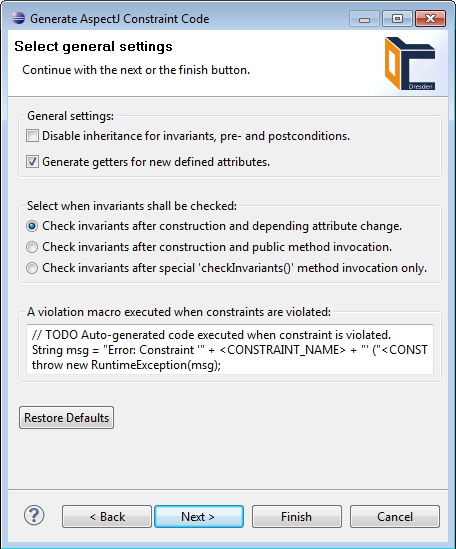
\includegraphics[width=0.9\linewidth]{figures/codegen/codegen04}
	\caption{The fourth step: general settings for the code generation.}
	\label{pic:codegen:codegen04}
\end{figure}

On the following page of the wizard we can specify general settings for the code
generation (cf. Fig.~\ref{pic:codegen:codegen04}). We can disable the 
inheritance of constraints (which would not be useful in our example because we 
want to enforce the constraint for \model{Persons}, but for \model{Students} and
\model{Professors} as well). We can also enable that the code generator will 
generate getter methods for newly defined attributes of \model{def} constraints.
More interesting is the possibility to select one of three provided strategies, 
when invariants shall be checked during runtime:

\begin{enumerate}
	\item Invariants can be checked after construction of an object and after any
	  change of an attribute or association which is in scope of the invariant
	  condition (\keyword{Strong Verification}).
	\item Invariants can be checked after construction of an object and before or 
	  after the execution of any public method of the constrained class
	  (\keyword{Weak Verification}).
	\item And finally, invariants can only be checked if the user calls a special 
	  method at runtime (\keyword{Transactional Verification}).
\end{enumerate}

These three scenarios can be useful for users in different situations. If a user
wants to verify strongly, that his constraints are verified after any change of 
any dependent attribute he should use \keyword{Strong Verification}. If he wants
to use attributes to temporary store values and constraints shall be verified if
any external class instance wants to access values of the constrained class
only,  he should use \keyword{Weak Verification}. If the user wants to work with
databases or other remote communication and the state of his constraint classes 
should be valid before data transmission only, he should use the strategy 
\keyword{Transactional Verification}.

Finally, we can specify a \keyword{Violation Macro} which specifies the code, 
which will be executed when a constraint is violated during runtime. By
default, the violation macro throws a run-time exception containing a message
saying which constraint was violated by which runtime object. Whithin such
messages, some specific keywords can be used to declare information such as the
violated constraint's name or body. Table~\ref{tab:codegen:patterns} gives an
overview over the allowed keywords and their meaning. We also want to have a
run-time exception thrown when our constraint is violated. Thus, we do not
change the violation macro and continue with the \eclipse{Next} button.

\begin{table}[h]
\begin{tabular}{|p{7cm}|p{7cm}|}
    \hline
    \textbf{Keyword} & \textbf{Meaning within generated error message} \\
    \hline
    \texttt{<CONSTRAINT\_NAME>} & 
    The name of the constraint violated during runtime. If the constraint has no
    name, the term \texttt{undefined} will be used instead.
    \\
    \hline
    \texttt{<CONSTAINTS\_BODY>} & 
    The body (\acs{OCL} expression) of the constraint violated during runtime.
    \\
    \hline
    \texttt{<OBJECT\_IN\_ILLEGAL\_STATE>} & 
    The Object causing the constraint violation at runtime. The keyword will be
    replaced by calling the \texttt{.toString()} method of the object.
    \\
    \hline
\end{tabular}
\caption{Keywords allowed to parameterize messages within violation macros.}
\label{tab:codegen:patterns}
\end{table}


\newpage
\subsection{Constraint-Specific Settings}

The last page of the code generation wizard provides the possibility to
configure some of the code generation settings constraint-specific by selecting
a constraint and adapting it's settings (cf.
Fig.~\ref{pic:codegen:codegen05}). We don't want to adapt the settings, thus 
we can finish the wizard and start the code generation by clicking the 
\eclipse{Finish} button.

\begin{figure}[!b]
	\centering
	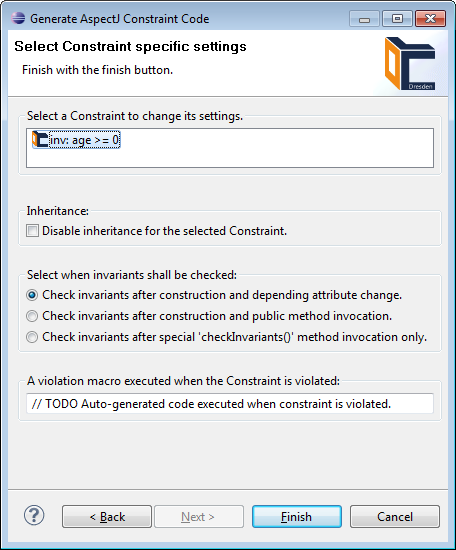
\includegraphics[width=0.9\linewidth]{figures/codegen/codegen05}
	\caption{The fifth step: constraint-specific settings for the code generation.}
	\label{pic:codegen:codegen05}
\end{figure}



\newpage
\section{The Generated Code}

After finishing the wizard, the code for the selected constraint will be 
generated. To see the result, we have to refresh our project in the workspace. 
We select the project 
\model{org.dresdenocl.\linebreak[0]examples.simple.constraint} in the
\eclipse{Package Explorer}, open the context menu and select the menu item 
\eclipse{Refresh}. Afterwards, our project contains a newly generated AspectJ 
file called 
\model{tu\-dres\-den\linebreak[0].ocl20\linebreak[0].pivot.examples.simple.constraints.InvAspect\-01.aj}
(cf. Fig.~\ref{pic:codegen:packageExplorer}). Now, we can rerun our JUnit test
case. The test case finishes successfully because the expected run-time 
exception is thrown (cf. Fig.~\ref{pic:codegen:junit02}).

\begin{figure}[!b]
	\centering
	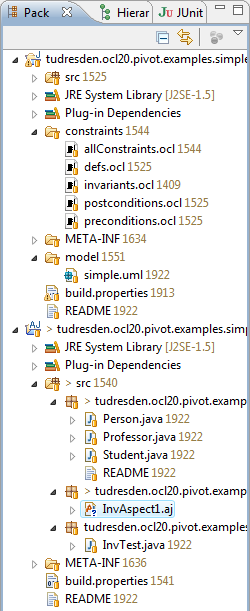
\includegraphics[width=0.45\linewidth]{figures/codegen/packageExplorer}
	\caption{The Package Explorer containing the newly generated AspectJ File.}
	\label{pic:codegen:packageExplorer}
\end{figure}


\begin{figure}[!t]
	\centering
	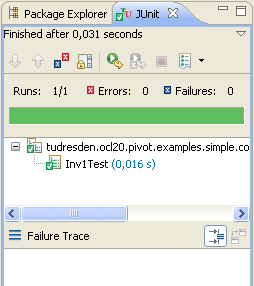
\includegraphics[width=0.45\linewidth]{figures/codegen/junit02}
	\caption{The successfully executed jUnit Test Case.}
	\label{pic:codegen:junit02}
\end{figure}


	
\section{Summary}
  
This chapter described how to generate AspectJ code using the
\keyword{OCL22Java} code generator of Dresden OCL. A more detailed
documentation of the OCL22Java code generator can be found in the Minor Thesis
(Gro�er Beleg) of Claas Wilke \cite{GB:Wilke}. Besides the use of OCL22Java via
Dresden OCL's GUI, you can also invoke OCL22Java via Dresden OCL's \acs{API}.
The easiest way to connect to Dresden OCL is via its \emph{Facade} providing
interfaces for all services of Dresden OCL. How to use Dresden OCL's facade is
documented in Chapter~\ref{chapter:integration}.
